\documentclass[usenames,dvipsnames,10pt]{beamer}
\usepackage[absolute,overlay]{textpos}

% Setup appearance:
\usetheme{Boadilla}
\usefonttheme[onlylarge]{structurebold}
\usecolortheme{seahorse}
\setbeamerfont*{frametitle}{size=\normalsize,series=\bfseries}
\setbeamertemplate{navigation symbols}{}
%\setbeamercolor{frametitle}{fg=Blue}
\renewcommand\alert[1]{{\color{Magenta} #1}}
\newcommand\program[1]{\texttt{#1}}

% Packages
\usepackage[english,ukrainian]{babel}
\usepackage{times}
\usepackage[T1]{fontenc}
\usepackage{color}
\usepackage{bm}
\usepackage{slashed}
\usepackage{booktabs}% http://ctan.org/pkg/booktabs
\usepackage{xspace}
\usepackage{multirow}
\usepackage{graphicx}
\newcommand{\tabitem}{~~\llap{\textbullet}~~}
\usepackage{minted}
\usepackage{scalerel}
\usepackage{amsmath}

\hypersetup{
	colorlinks=true,
	linktoc=page,
	citecolor=Blue,
	linkcolor=Blue,
	urlcolor=Blue 
}

\setlength{\fboxsep}{0pt}%
\setlength{\fboxrule}{1pt}%

%\definecolor{stcoupcolor}{RGB}{255,0,51}

% Setup TikZ
\usepackage{tikz}
\usetikzlibrary{arrows,shapes,backgrounds,positioning}
\tikzstyle{block}=[draw opacity=0.7,line width=1.4cm]

% arrows
\tikzset{
    myarrow/.style={
        draw,
        fill=orange,
        single arrow,
        rounded corners=1,
        %        width=2ex,
        minimum width=2ex,
        minimum height=3ex,
        single arrow head extend=1ex
    }
}
\newcommand{\arrowup}{\tikz [baseline=-0.5ex]{\node [myarrow,rotate=90] {};}}
\newcommand{\arrowdown}{\tikz [baseline=-0.5ex]{\node [myarrow,rotate=-90] {};}}
\newcommand{\arrowright}{\tikz [baseline=-0.5ex]{\node [myarrow,rotate=0] {};}}
\newcommand{\arrowleft}{\tikz [baseline=-0.5ex]{\node [myarrow,rotate=180] {};}}

% draw connection
\newcommand{\tikzmark}[1]{\tikz[remember picture] \node[coordinate] (#1) {#1};}

% page numbering (backup)
\newcommand{\backupbegin}{\newcounter{finalframe}\setcounter{finalframe}{\value{framenumber}}}
\newcommand{\backupend}{\setcounter{framenumber}{\value{finalframe}}}

% Author, Title, etc.
\title[Вимірювання перерізів. Розділення сигналу і фону]{\large Вимірювання перерізів. Розділення сигналу і фону}
\author[Олександр Зенаєв]{Олександр Зенаєв}
\date{}

% block with custom width
\newenvironment<>{varblock}[2][.9\textwidth]{%
    \setlength{\textwidth}{#1}
    \begin{actionenv}#3%
        \def\insertblocktitle{#2}%
        \par%
        \usebeamertemplate{block begin}}
    {\par%
        \usebeamertemplate{block end}%
\end{actionenv}}

\setbeamertemplate{itemize/enumerate body begin}{\footnotesize}
\setbeamertemplate{itemize/enumerate subbody begin}{\footnotesize}

\tikzset{
    every overlay node/.style={
        rounded corners,anchor=north west,
    },
}
\def\tikzoverlay{%
    \tikz[baseline,overlay]\node[every overlay node]
}%

% main part
\begin{document}
    \begin{frame}[plain]
    %\centering\includegraphics[width=0.15\textwidth]{pics/logo/cms.png}
    %\hspace{0.1\textwidth}
    %\centering\includegraphics[width=0.18\textwidth]{pics/logo/h1}
    %\hspace{0.1\textwidth}
    %\centering\includegraphics[width=0.15\textwidth]{pics/logo/desyNEW}
    %\hspace{0.1\textwidth}
    %\centering\includegraphics[width=0.15\textwidth]{pics/logo/zeus}
    %\hspace{0.1\textwidth}
    %\centering\includegraphics[width=0.15\textwidth]{pics/logo/xFitterLogo1.png}
    
    \vspace{-0.05\textheight}
    \titlepage
    
    %\vspace{-0.15\textheight}
    %\centering\includegraphics[width=0.4\textwidth]{pics/titlepic.jpg}

    %\vspace{-0.15\textheight}
    %{\color{blue} Overview:}
    
    \vspace{0.04\textheight}
    \centering
    %place \\
    %date
\end{frame}

% number of slides w/out backup
\renewcommand{\inserttotalframenumber}{2}
\setbeamercolor{footline}{fg=blue}
\setbeamerfont{footline}{series=\bfseries}

\begin{frame}
	\frametitle{Переріз народження (визначення)}
	\begin{itemize}
		\item Переріз народження, або переріз реакції (production cross section, or just cross section, x-section, $\sigma$) -- фізична величина, яка характеризує ймовірність утворення певного процесу або реакції у зіткненнях частинок
		\item Переріз народження визначає частоту подій певного типу (наприклад, народження нових частинок). Його можна уявити як ефективну площу, яку ``бачать'' частинки, що взаємодіють певним чином
		\item Переріз вимірюється в одиницях площі {\it барн (barn, b)}: $1 \mathrm{b} = 10^{-24} \mathrm{cm}^2$. У HEP зазвичай використовують $1 \mathrm{mb} = 10^{-27}\mathrm{cm}^2$, $1\mathrm{\mu b} = 10^{-30}\mathrm{cm}^2$ \dots $1 \mathrm{fb} = 10^{-39} \mathrm{cm}^2$
		\item Переріз визначається за формулою:
		\begin{equation*}
			\sigma = \frac{N}{L},
		\end{equation*}
		де $N$ -- кількість подій, $L$ -- світимість (luminosity, іноді позначають $\mathcal{L}$)
		\item $L$ характеризує кількість зіткнень частинок у точці взаємодії та визначається параметрами пучків частинок (інтенсивністю, частотою зіткнень тощо), вимірюється в $\mathrm{b}^{-1}$ (inversed barn) або $\mathrm{cm}^{-2}$
		\item Розрізняють миттєву світимість (instantaneous luminosity) за одиницю часу (наприклад, для LHC Run-3 це приблизно $10^{34} \mathrm{cm}^{-2}\mathrm{s}^{-1}$), та інтегральну світимість (integrated luminosity) за певний час, яка визначає, скільки всього було накопичено даних в експерименті (наприклад, з початку 2024 р. і до вересня ATLAS і CMS накопичили близько $100 \mathrm{fb}^{-1}$)
	\end{itemize}
\end{frame}

\begin{frame}
	\frametitle{Вимірювання перерізу народження}
	\begin{itemize}
		\item Для експериментального вимірювання перерізу використовується та сама формула:
		\begin{equation*}
			\sigma = \frac{N}{L}
		\end{equation*}
		\item Втім, ${N}$ може містити не тільки сигнал, але і фон: 
		\begin{equation*}
		N_s = N - N_{bg}
		\end{equation*}
			Фон або віднімається за передбаченням, або визначається через template fitting
		\item Крім того, не всі події можуть бути зареєстровані
		\begin{equation*}
			N_s = N_s^{rec}/\epsilon
		\end{equation*}
		Ефективність реєстрації $\epsilon$ визначається з Монте-Карло (МК) симуляції
		\item Іноді розрізняють аксептанс ($A$) як частину подій, яка геометрично потрапляє в детектор, і ефективність реєстрації ($\epsilon$) подій детектором (сюди також можуть входити обмеження, що накладаються для зменшення фону)
		\item Більш повна формула для обрахунку перерізу:
		\begin{equation*}
		\sigma = \frac{N-N_{Bg}}{\epsilon \cdot A \cdot L},
		\end{equation*}
		\end{itemize}
\end{frame}

\begin{frame}
	\frametitle{Визначення кількості сигнальних подій $N_s$}
	Задача: є $N$ подій. Треба визначити частки сигналу ($N_s$) і фону ($N_{bg}$).
	\begin{itemize}
		\item[(1)] відняти очікувану кількість фонових подій
		\begin{itemize}
			\item потребує знання перерізу фонових подій
			\item симулюють фонові події, використовуючи певну модель, далі симулюють взаємодію частинок з детектором, проводять реконструкцію подій, визначають $N_{Bg}$ і потім $N_s = N - N_{bg}$
			\item  результат залежить від моделі (model dependence), яку використовували для симуляції фону (кінематичні розподіли)
			\item рідко використовується в чистому вигляді, оскільки фон у HEP експериментах занадто складний і містить багато компонент
		\end{itemize}
		\item[(2)] шаблонна підгонка (template fitting)
		\begin{itemize}
			\item одним із варіантів є реконструкція і фітування розподілу інваріантної маси 
			\item в цьому випадку $N_s$ визначається як площа піку
			\item функція для опису комбінаторного фону зазвичай підбирається емпірично (data driven) і може варіюватися для оцінки систематичної похибки
			\item чим менший фон, тим менша буде статистична похибка $\Delta N_s$
		\end{itemize}
	\end{itemize}
	
	\vspace{0.02\textheight}
	\footnotesize
	\begin{tabular}{|l|l|l|}
		\hline
		Method & Statistical uncertainty & Model dependence \\ \hline
		Background subtraction & $\Delta N_s = \sqrt{N_s}$ & $+$ \\
		Template fitting & $\Delta N_s \sim \sqrt{N_s + N_{Bg}}$ & $-$ \\
		\hline
	\end{tabular}
	
	\vspace{0.02\textheight}
	N.B. Можуть бути інші специфічні методи, такі як віднімання фону через використання подій з неправильним електричним зарядом та ін.
\end{frame}

\begin{frame}
	\frametitle{Визначення кількості сигнальних подій $N_s$}
	\centering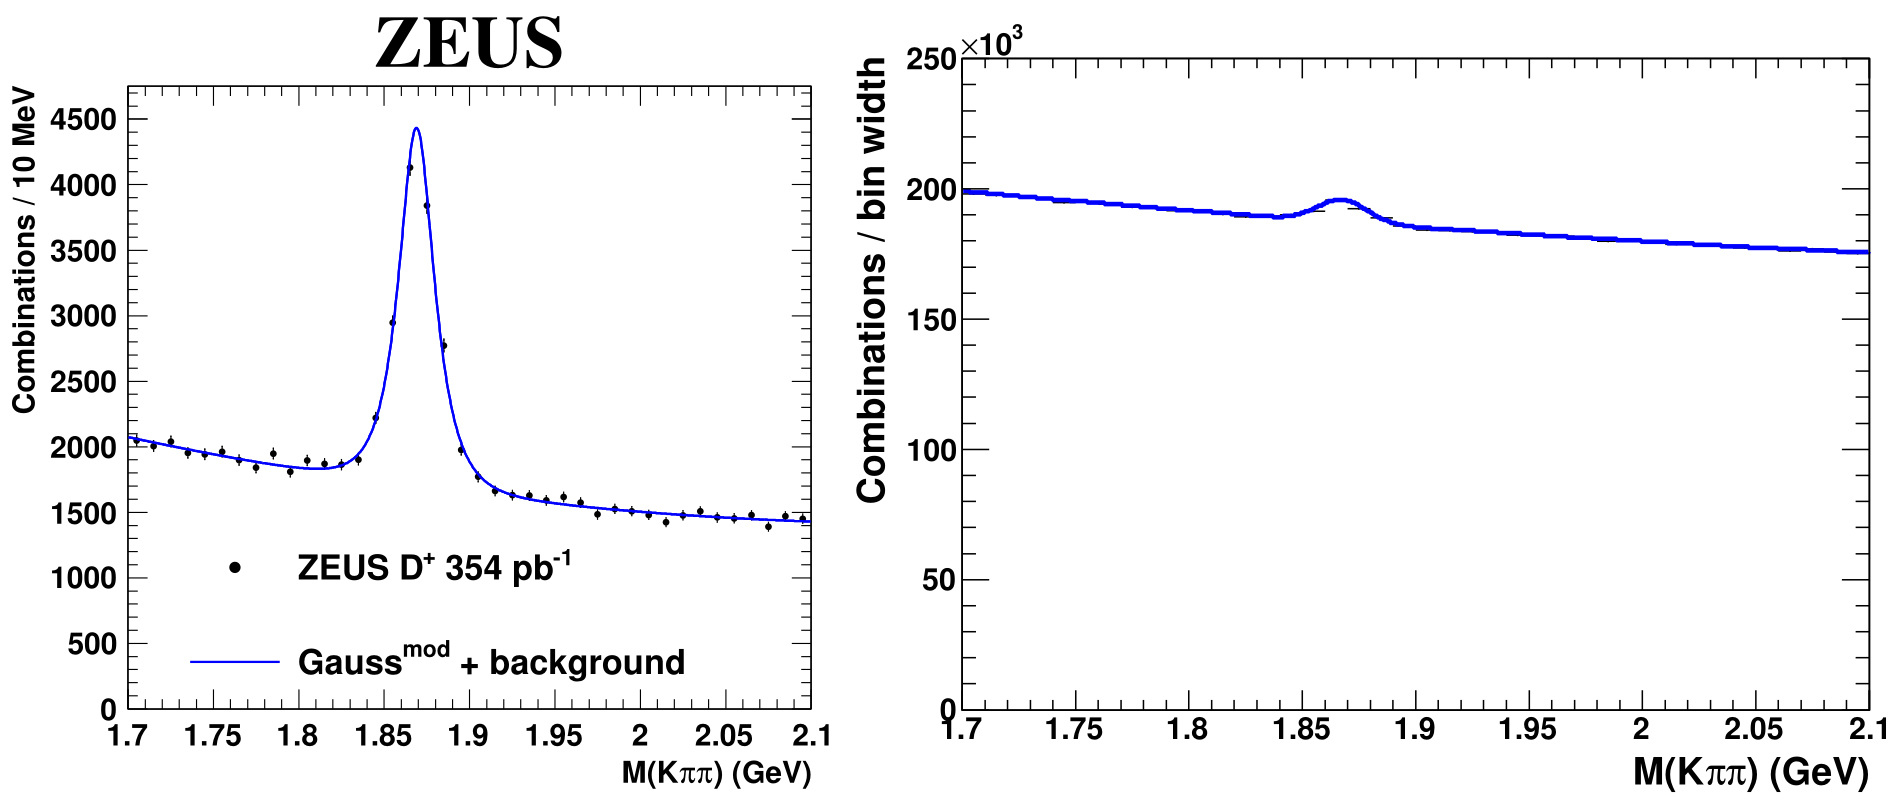
\includegraphics[width=0.45\textwidth,clip = true, trim = 0 0 1070 0]{pics/zeus_dplus_mass.png}
	\centering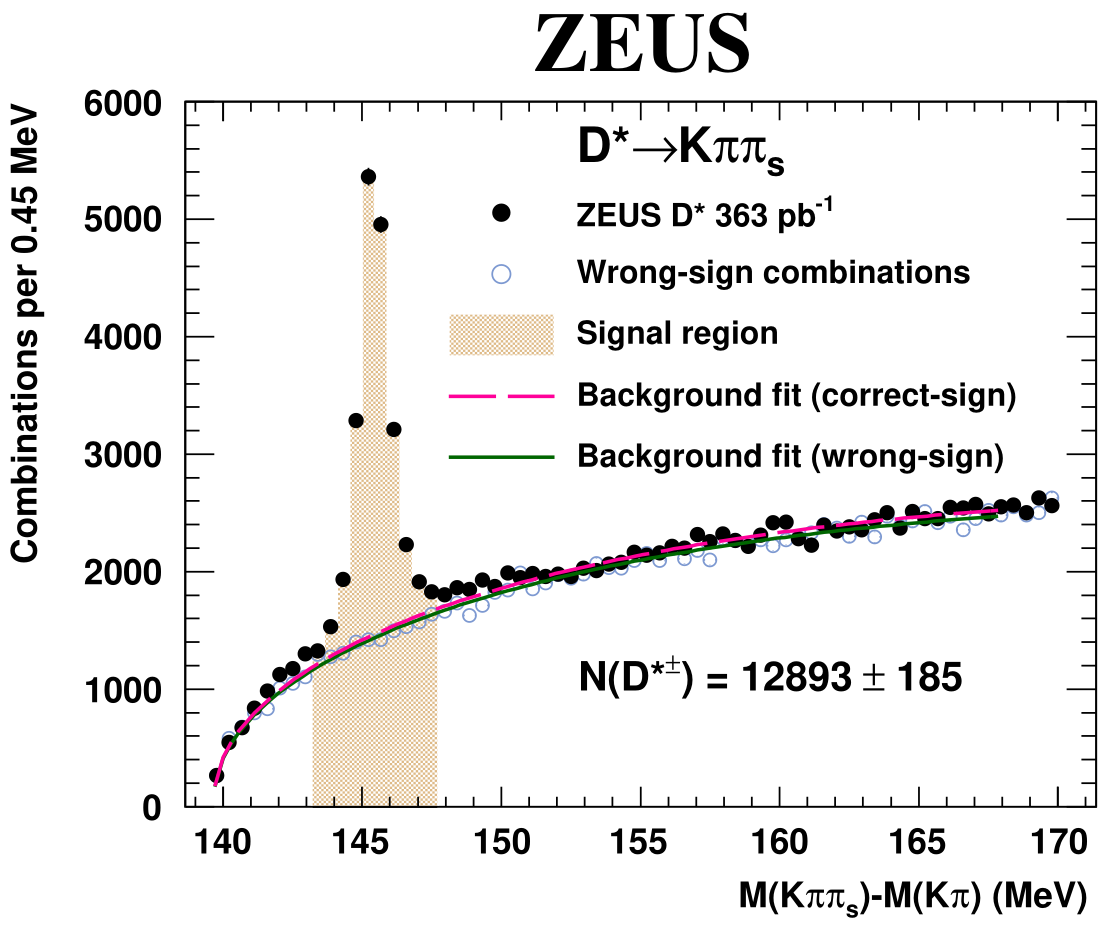
\includegraphics[width=0.53\textwidth]{pics/zeus_dstar_mass.png}
	
	\begin{itemize}
		\item left: ``Measurement of $D^{\pm}$	production in deep inelastic $ep$ scattering with the ZEUS detector at HERA'': fitting of invariant mass distribution $D^{+} \to K^{-}\pi^{+}\pi^{+}$ \newline \href{https://inspirehep.net/literature/1220382}{[JHEP 05 (2013) 023, arXiv:1302.5058]}
		\item right: ZEUS Coll., ``Measurement of $D^{*\pm}$ production in deep inelastic scattering at HERA'': wrong sign $D^{*+} \to D^0(\to K^{+}\pi^{-})\pi_s^{+}$  subtraction from correct sign $D^{*+} \to D^0(\to K^{-}\pi^{+})\pi_s^{+}$ \newline \href{https://inspirehep.net/literature/1225526}{[JHEP 05 (2013) 097, arXiv:1303.6578]}
	\end{itemize}
\end{frame}

\begin{frame}
	\frametitle{Розділення сигналу і фону}
	Задача: є $N$ подій. Відсіяти якомога більше фонових подій і залишити якомога більше сигнальних подій, щоб мінімізувати $\Delta N_s / N_s$ (задача класифікації)
	\begin{itemize}
		\item Найважливіша складова аналізу даних: дозволяє ``побачити'' кілька (десятків, сотень, тисяч) сигнальних подій серед мільярдів усіх зареєстрованих подій
		\item Найпростіший підхід: накладати обмеження (cuts) на кінематичні властивості подій та/або окремих реконструйованих частинок (імпульси, кути)
		\item Більш сучасний метод: алгоритми машинного навчання (дерева рішень та ін.)
		\item Маємо $N$ подій, що містять сигнал і фон ($N = N_{s}+N_{b}$). Із них відбираємо $N^{sel}$ подій, які також будуть містити фон і сигнал ($N^{sel} = N^{sel}_{s}+N^{sel}_{b}$). Результат характеризується ефективністю (efficiency, $\epsilon$) та чистотою (purity, $p$):
	\end{itemize}
	\begin{columns}
		\column{0.4\textwidth}
		\begin{align*}
			\epsilon &= \frac{N^{sel}_{s}}{N_{s}}\\
			p &= \frac{N^{sel}_{s}}{N^{sel}_{s}+N^{sel}_{b}}
		\end{align*}
		\column{0.6\textwidth}
		\centering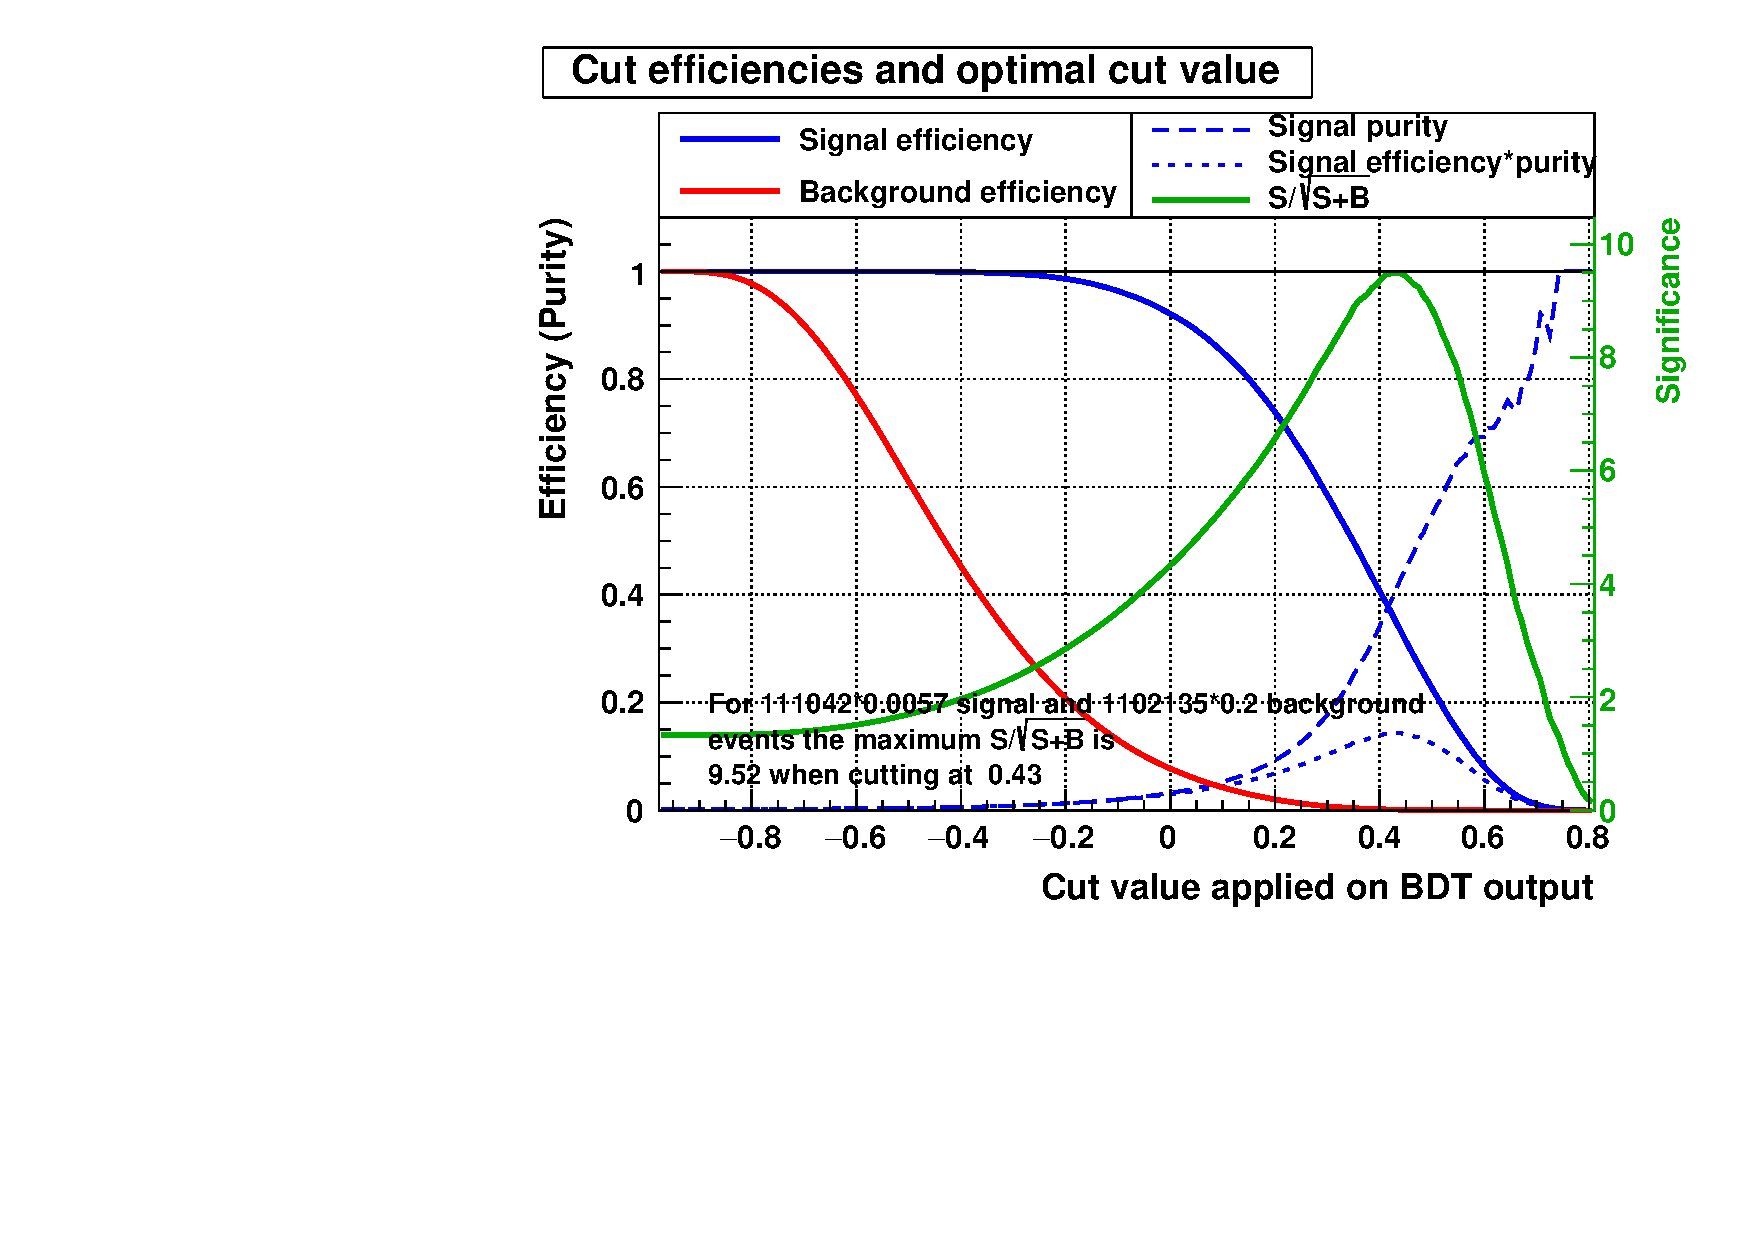
\includegraphics[width=0.8\textwidth]{pics/mvaeffs_BDT.pdf}
	\end{columns}
\end{frame}

\begin{frame}
\frametitle{Практичне заняття}
\begin{itemize}
	\item Використовуючи генератор подій, згенерувати додатковий комбінаторний фон (декілька $\pi^{\pm}$)
	\item Накладаючи обмеження на імпульси частинок, зменшити фон
	\item Визначити ефективність та чистоту
	\item Визначити переріз народження, скоректований на ефективність відбору подій
\end{itemize}

{\footnotesize 
\vspace{0.05\textheight}
Github:\newline \url{https://github.com/zenaiev/hep/blob/main/invmass/invmass_adv.py}

\vspace{0.05\textheight}
Google Colab:\newline \scalebox{0.98}{\url{https://colab.research.google.com/github/zenaiev/hep/blob/main/invmass/invmass_adv.ipynb}}
}
\end{frame}

%\begin{frame}
%\frametitle{Status of xFitter releases}
%\begin{columns}\column{\dimexpr\paperwidth-10pt}
%\centering{\includegraphics[width=1.0\textwidth]{pics/pic.png}}
%\end{columns}
%\end{frame}

%\appendix
%\backupbegin
%\begin{frame}
%\frametitle{}
%\centering{\Huge \bf BACKUP}
%\end{frame}
%\backupend

\end{document}
